%=================================================================
\documentclass[Universe,article,submit,moreauthors,pdftex]{Definitions/mdpi} 
%=================================================================
\firstpage{1} 
\makeatletter 
\setcounter{page}{\@firstpage} 
\makeatother
\pubvolume{xx}
\issuenum{1}
\articlenumber{5}
\pubyear{2020}
\copyrightyear{2020}
%\externaleditor{Academic Editor: Roman Pasechnik}

%\preto{\abstractkeywords}{\nolinenumbers} %>>>>nolinenumbers<<<
%\history{Received: 10 September 2020; Accepted: date; Published: date}
%\updates{yes} % If there is an update available, un-comment this line

%% MDPI internal command: uncomment if new journal that already uses continuous page numbers 
%\continuouspages{yes}

%------------------------------------------------------------------
% The following line should be uncommented if the LaTeX file is uploaded to arXiv.org
\pdfoutput=1

%=================================================================
% Add packages and commands here. The following packages are loaded in our class file: fontenc, inputenc, calc, indentfirst, fancyhdr, graphicx,epstopdf, lastpage, ifthen, lineno, float, amsmath, setspace, enumitem, mathpazo, booktabs, titlesec, etoolbox, tabto, xcolor, soul, multirow, microtype, tikz, totcount, amsthm, hyphenat, natbib, hyperref, footmisc, url, geometry, newfloat, caption

%=================================================================
%% Please use the following mathematics environments: Theorem, Lemma, Corollary, Proposition, Characterization, Property, Problem, Example, ExamplesandDefinitions, Hypothesis, Remark, Definition, Notation, Assumption
%% For proofs, please use the proof environment (the amsthm package is loaded by the MDPI class).

%=================================================================
% Full title of the paper (Capitalized)
\Title{\uppercase{Electron Positron Partition Function in Early Universe}}

% Author Orchid ID: enter ID or remove command
\newcommand{\orcidauthorA}{0000-0001-8217-1484} % Add \orcidA{} behind the author's name
\newcommand{\orcidauthorB}{0000-0001-5038-8427} % Add \orcidB{} behind the author's name
 
% Authors, for the paper (add full first names)
\Author{Johann Rafelski, Cheng Tao Yang, and Andrew Steinmetz}
% Authors, for metadata in PDF
\AuthorNames{Firstname Lastname, and Firstname Lastname}

% Affiliations / Addresses (Add [1] after \address if there is only one affiliation.)
\address[1]{%
Department of Physics, The University of Arizona, Tucson, Arizona 85721, USA} 

% Contact information of the corresponding author
\corres{Correspondence: JohannR@Arizona.EDU
%; %Tel.: (optional; include country code; if there are multiple corresponding authors, add author initials) +xx-xxxx-xxx-xxxx (F.L.)
}

% Current address and/or shared authorship
%\firstnote{Current address: Affiliation 3} 
%\secondnote{These authors contributed equally to this work.}
% The commands \thirdnote{} till \eighthnote{} are available for further notes

%\simplesumm{} % Simple summary

%\conference{} % An extended version of a conference paper

% Abstract (Do not insert blank lines, i.e. \\) 

\abstract{We will write abstract here}
%
\keyword{Magnetization; Electron-Positron plasma; Cosmology.}
%%%%%%%%%%%%%%%%%%%%%%%%%%%%%%%%%%%%%%%%%%
\begin{document}
%%%%%%%%%%%%%%%%%%%%%%%%%%%%%%%%%%%%%%%%%% 
\section{Introduction}
\noindent The electron-positron epoch of the early universe was home to several significant events which have greatly shaped our contemporary universe including neutrino decoupling, Big Bang Nucleosynthesis (BBN), and the annihilation of most electrons and positrons partially reionizing the universe as well as setting the stage for the eventually recombination period which would generate the cosmic microwave background (CMB). Therefore, correctly describing the dynamics of this $e^{+}e^{-}$ plasma is of interest when considering modern mysteries such as the origin of cosmic extra-galactic magnetic fields. While most approaches tackle magnetized plasmas from the perspective of magnetohydrodynamics (MHD), a primarily classical or semi-classical approach, our perspective is to demonstrate that fundamental quantum statistical analysis can lead to further insights on the behavior of magnetized plasmas.

The universe is filled with magnetic fields at various scales and strengths both within galaxies and in deep inter-galactic space far and away from matter sources. Extragalactic magnetic fields are not well constrained today, but are required by observation to be non-zero with a magnitude between $10^{-20}\ \mathrm{T}<B_{relic}<10^{-12}\ \mathrm{T}$ over Mpc coherent length scales. The upper bound is contrained from the characteristics of the CMB while the lower bound is contrained by nonobservation of ultra-energetic photons from blazars. There are generally two considered origins for extragalactic magnetic fields: (a) matter-induced dynamo processes involving Amperian currents and (b) primordial (or relic) seed magnetic fields whose origins may go as far back as the Big Bang itself. It is currently unknown which origin accounts for extragalactic magnetic fields today or if it some combination thereof. Even if magnetic fields in the universe today are primarily driven via amplification through Amperian matter currents, such models still require primordial seeds fields at some point to act as catalyst.
\begin{figure}[t]
  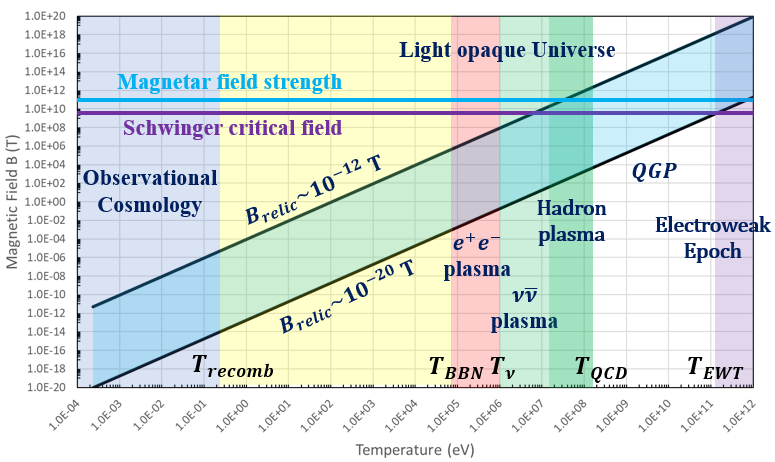
\includegraphics[scale=0.75]{relic_plot.PNG}
  \label{fig1}
  \caption{Qualitative value of the primordial magnetic field over the evolutionary lifespan of the universe. As magnetic flux is conserved over comoving surfaces, the primordial relic field is expected to dilute as $\approx1/a(t)^{2}$ meaning the contemporary small bound values of $5\times10^{-12}\ \mathrm{T}>B_{relic}>10^{-20}\ \mathrm{T}$ may have once represented large magnetic fields in the early universe. This is relic magnetic field would then be generated by the last phase of significant magnetization in the early universe. This figure is meant to be illustrative and it is unlikely the magnetization of the universe would proceed unhindered and unaltered into the ultra-dense plasma phases of the early universe. The values of the Schwinger critical field and the upper bound of surface magnetar field strength are included for scale.}
  \centering
\end{figure}
We then connect back to the plasmas of the early universe as such primordial fields would be lensed through the various plasmas that existed when the universe was far hotter and denser. Of particular interest to us is the electron-positron plasma which existed in the early universe at temperature $T>20\ \mathrm{KeV}$ which was the last plasma in the universe where the madium density was many orders of magnitude above ordinary lab atomic density. It it in this dense plasma environment that BBN occured and where similar plasmas can still be found within exotic stars such as magnetars.
%%%%%%%%%%%%%%%%%%%%%%%%%%%%%%%%%%%%%%%%%%%%%%%%%%%%%%%%%%%%%%%%%%%
\section{Energy Eigenvalues}\label{sec:energy}
\noindent As a starting point, we consider the energy-eigenvalues of charged fermions within a homogenous magnetic field. Here, we have several choices: We could assume the typical Dirac energy eigen-values with gyromagnetic g-factor set to $g=2$. But as electrons, positrons and most plasma species have anomalous magnetic moments (AMM), we require a more complete model. Another option would be to modify the Dirac equation with a Pauli term, often called the Dirac-Pauli (DP) approach, via
\begin{align}
  \label{Pauli} \hat{H}_{\mathrm{AMM}} = -a\frac{e}{2m}\frac{\sigma_{\mu\nu}F^{\mu\nu}}{2}\,,
\end{align}
where $\sigma_{\mu\nu}$ is the spin tensor proportional to the commutator of the gamma matrices and $F^{\mu\nu}$ is the EM field tensor. The AMM is defined via g-factor as
\begin{align}
  \label{Pauli} \frac{g}{2}=1+a\,.
\end{align}
This approach, while straightforward, would complicate the energies making analytic understanding and clarity difficult without a clear benefit. Our preferred model for the AMM is through the Klein-Gordon-Pauli (KGP) equation which is given by
\begin{alignat}{1}
  \label{KGP} \left(\left(i\partial_{\mu}-eA_{\mu}\right)^{2}-m^{2}-e\frac{g}{2}\frac{\sigma_{\mu\nu}F^{\mu\mu}}{2}\right)\Psi=0\,.
\end{alignat}
We wish to emphasize, that each of the three above models are distict and have differing physical consequences and are not interchangable. One benefit of the KGP approach is that the energies take eigenvalues which are mathematically similar to the Dirac energies. Considering the $e^\pm$ plasma in a uniform magnetic field $B$ pointing along the $z$-axis, the energy of $e^\pm$ fermions can be written as
\begin{align}
  \label{KGPEnergy} E_{n}^{s}&=\sqrt{p^2_z+\tilde{m}^2+2eBn},\qquad\tilde{m}^2=m^2_e+eB\left(1-gs\right),\qquad s=\pm\frac{1}{2},\qquad n=0,1,2,3,\dots
\end{align}
Here we introduce a notion of \lq\lq magnetic mass\rq\rq\ which inherents the spin-specific part of the energies adding them to the mass. This convention is also generalizable to further non-minimal electromagnetic models with more exotic energy contributions such that we write
\begin{align}
  \label{MagMass} m^{2}\rightarrow\tilde{m}^2(B)\,.
\end{align}
This definition also pulls out the ground state Landau energy separating it from the remainder of the Landau tower of states. One restriction is that the magnetic-mass must remain positive definite in our analysis thus we require
\begin{align}
  \label{MagMass} \tilde{m}^2(B)=m^2_e+eB\left(1-gs\right)>0\,.
\end{align}
This condition fails under ultra-strong magnetic fields of order
\begin{align}
  \label{MagMassFail} B_{\mathrm{crit}}=\frac{m^{2}}{ea}=\frac{\mathcal{B}_{S}}{a}\approx3.8\times10^{12}\ \mathrm{T}\,,
\end{align}
where $\mathcal{B}_{S}$ is the Schwinger critical field strength. For electrons, this field strength is well above the window of magnetic field stregnths of interest during the late $e^{+}e^{-}$ epoch.

%%%%%%%%%%%%%%%%%%%%%%%%%%%%%%%%%%%%%%%%%%%%%%%%%%%%%%%%%%%%%%%%%%%
\section{Partition function}
\noindent We turn our attention now to the statistical behavior of the $e^{+}e^{-}$ system. We can utilize the Fermion partition function given by
\begin{align}
  \label{PartFunc} \ln(\mathcal{Z})=\sum_{\alpha}\ln\left(1+e^{-\beta(E-\eta)}\right)\,,
\end{align}
where $\beta=1/T$, $\alpha$ is the set of quantum numbers in the system, and $\eta$ is the generalized chemical potential. The magnetized $e^{+}e^{-}$ system should be considered a system of four quantum species: Particles and anti-particles, and spign aligned and anti-aligned.
 
If we consider a system that all electrons and positrons are spin aligned and antialigned with the magnetic field $B$, then the partition function of the system can be written as
\begin{align}
\ln\mathcal{Z}_{tot}=\frac{2eBV}{(2\pi)^2}\sum_{n=0}^\infty\int^\infty_{0} \!\!dp_z\bigg[\ln\left(1+e^{-\beta(E_{n}^\pm-\mu_e)}\right)+\ln\left(1+e^{-\beta(E_{n}^\pm+\mu_e)}\right)\bigg],
\end{align}
where $\mu_e$ is the chemical potential of electron, and energy $E_{n}^\pm$ can be written as
\begin{align}
E_{n}^\pm&=\sqrt{p^2_z+\tilde m^2_\pm+2eBn},\qquad\tilde{m}^2_\pm=m^2_e+eB\left(1\pm\frac{g}{2}\right).
\end{align}

To simplify the partition function we can consider the expansion of the logarithmic function, we have
\begin{align}
\ln\left(1+x\right)=\sum^{\infty}_{k=1}\frac{(-1)^{k+1}}{k}x^k, \,\,\,\,\,\,\,\mathrm{for}\,|x|<1.
\end{align}
Then the partition function of electron/positron system can be written as
\begin{align}
\ln\mathcal{Z}_{tot}=&\frac{2eBV}{(2\pi)^2}\sum_{n=0}^\infty\int^\infty_{0} \!\!dp_z\sum^{\infty}_{k=1}\frac{(-1)^{k+1}}{k}\bigg[e^{k\beta\mu_e}+e^{-k\beta\mu_e}\bigg]e^{-k\beta E_n^\pm}\notag\\
&=\frac{2eBV}{(2\pi)^2}\sum_{n=0}^\infty\sum^{\infty}_{k=1}\frac{(-1)^{k+1}}{k}\bigg[2\cosh{(k\beta\mu_e)}\bigg]\int_0^\infty dp_z\,e^{-k\beta E_n^\pm}\notag\\
&=\frac{2eBTV}{(2\pi)^2}\sum^{\infty}_{k=1}\frac{(-1)^{k+1}}{k^2}\bigg[2\cosh{(k\beta\mu_e)}\bigg]\sum_{n=0}^\infty W^\pm_1(n),
\end{align}
where we introduce the function $W^\pm_1(n)$ as follows
\begin{align}
W^\pm_1(n)\equiv\frac{k\sqrt{\tilde{m}^2_\pm+2eBn}}{T}\,\,K_1\!\!\left({k\sqrt{\tilde{m}^2_\pm+2eBn}}/{T}\right).
\end{align}

Considering the Euler-Maclaurin formula to replace the sum over Landau levels, we have
\begin{align}
\sum^{\infty}_{n=0}W^\pm_1(n)=\int^\infty_0\!\!dn\,W^\pm_1(n)+\frac{1}{2}\bigg[W^\pm_1(\infty)+W^\pm_1(0)\bigg]+\frac{1}{12}\bigg[\left.\frac{\partial W^\pm_1}{\partial n}\right|_{\infty}-\left.\frac{\partial W^\pm_1}{\partial n}\right|_{0}\bigg]+R
\end{align}
where $R$ is the error remainder which is defined by integrals over Bernoulli polynomials. Using the properties of Bessel function we obtain
\begin{align}
\sum^{\infty}_{n=0}W^\pm_1(n)&=\int^\infty_0\!\!dn\,W^\pm_1(n)+\frac{1}{2}W^\pm_1(0)-\frac{1}{12}\left.\frac{\partial W^\pm_1}{\partial n}\right|_{0}+R\\
&=\left(\frac{T^2}{k^2eB}\right)\left[\left(\frac{k\tilde{m}_\pm}{T}\right)^2K_2(k\tilde m_\pm/T)\right]+\frac{1}{2}\left[\left(\frac{k\tilde{m}_\pm}{T}\right)K_1(k\tilde m_\pm/T)\right]+\frac{1}{12}\left[\left(\frac{k^2eB}{T^2}\right)K_0(k\tilde m_\pm/T)\right]+R.
\end{align}
Replacing the sum over Landau levels by the integral, the partition function becomes
\begin{align}
&\ln\mathcal{Z}_{tot}=\ln\mathcal{Z}_{free}+\ln\mathcal{Z}_B+\ln\mathcal{Z}_R
\end{align}
where we defined 
\begin{align}
&\ln\mathcal{Z}_{free}=\frac{2T^3V}{(2\pi)^2}\sum^{\infty}_{k=1}\frac{(-1)^{k+1}}{k^4}\cosh{(k\mu_e/T)}\left[\left(\frac{k\tilde{m}_\pm}{T}\right)^2K_2(k\tilde m_\pm/T)\right]\\
&\ln\mathcal{Z}_B=\frac{4eBTV}{(2\pi)^2}\sum^{\infty}_{k=1}\frac{(-1)^{k+1}}{k^2}\cosh{(k\mu_e/T)}\bigg[\frac{k\tilde{m}_\pm}{2T}K_1(k\tilde m_\pm/T)+\frac{k^2eB}{12T^2}K_0(k\tilde m_\pm/T)\bigg]\\
&\ln\mathcal{Z}_R=\frac{4eBTV}{(2\pi)^2}\sum^{\infty}_{k=1}\frac{(-1)^{k+1}}{k^2}\cosh{(k\mu_e/T)}R
\end{align}
 
For nonrelativistic electron-positron plasma, we can consider the partition function in Boltzmann approximation and assuming the error remainder $R$ is small and can be neglected. In this case, we have
\begin{align}
\ln\mathcal{Z}_{tot}=&\frac{T^3V}{(2\pi)^2}\left[2\cosh(\mu_e/T)\right]\left(\frac{\tilde m_\pm}{T}\right)^{\!\!2} K_2(\tilde m_\pm/T)\notag\\
&+\frac{2eBTV}{(2\pi)^2}\left[2\cosh(\mu_e/T)\right]\left[\frac{1}{2}\left(\frac{\tilde m_\pm}{T}\right)K_1(\tilde m_\pm/T)+\frac{1}{12}\left(\frac{eB}{T^2}\right)K_0(\tilde m_\pm/T)\right]
\end{align}
It can be written as
\begin{align}\label{lnZ}
\ln\mathcal{Z}_{tot}=\frac{T^3V}{(2\pi)^2}\left[2\cosh(\mu_e/T)\right]\left\{\left(\frac{\tilde m_\pm}{T}\right)^{\!\!2} K_2(\tilde m_\pm/T)+\frac{eB}{T^2} \left[\left(\frac{\tilde m_\pm}{T}\right)K_1(\tilde m_\pm/T)+\frac{1}{6}\left(\frac{eB}{T^2}\right)K_0(\tilde m_\pm/T)\right]
\right\}
\end{align}

%%%%%%%%%%%%%%%%%%%%%%%%%%%%%%%%%%%%%%%%%%%%%%%%%%%%%%%%%%%%%%%%%%
\section{Chemical potential and Magnetization}

%~~~~~~~~~~~~~~~~~~~~~~~~~~~~~~~~~~~~~~~~~~~~~~~~~~~~~~~~~~~~~~~~~~~~~~~~~~~~~~~~~~~~~~~~~~~~~~~~~~~~~~~~~

\subsection{Charge neutrality}
Giving the partition function in Boltzmann limit Eq.(\ref{lnZ}) the net number density of electron can be written as
\begin{align}
\left(n_e-n_{\bar e}\right)&=\frac{T}{V}\frac{\partial}{\partial \mu_e}\ln\mathcal{Z}_{tot}\notag\\
&=\frac{2T^3}{(2\pi)^2}\sinh{(\mu_e/T)}\left[\left(\frac{\tilde{m}_\pm}{T}\right)^2K_2(\tilde m_\pm/T)\right]\notag\\&
\qquad+\frac{4eBT}{(2\pi)^2}\sinh{(\mu_e/T)}\bigg[\frac{\tilde{m}_\pm}{2T}K_1(\tilde m_\pm/T)+\frac{eB}{12T^2}K_0(\tilde m_\pm/T)\bigg]
\end{align}
Using the charge neutrality, we have
\begin{align}
n_p&=\left(n_e-n_{\bar e}\right)\notag\\
&=\frac{2T^3}{(2\pi)^2}\sinh{(\mu_e/T)}\left[\left(\frac{\tilde{m}_\pm}{T}\right)^2K_2(\tilde m_\pm/T)\right]\notag\\
&\qquad+\frac{4eBT}{(2\pi)^2}\sinh{(\mu_e/T)}\bigg[\frac{\tilde{m}_\pm}{2T}K_1(\tilde m_\pm/T)+\frac{eB}{12T^2}K_0(\tilde m_\pm/T)\bigg]
\end{align}
where $n_p$ is the number density of proton. It is also convenient to introduce the dimensionless variables:
\begin{align}
x_\pm=\frac{\tilde m_\pm}{T},\qquad b_0=\frac{eB}{T^2}
\end{align}
and we obtain
\begin{align}
n_p&=\frac{T^3}{(2\pi)^2}\left[2\sinh{(\mu_e/T)}\right]\left[x_\pm^2K_2(x_\pm)+b_0x_\pm K_1(x_\pm)+\frac{b^2_0}{6}K_0(x_\pm)\right]
\end{align}
In this case, given the magnetic field $B$ we can solve the chemical potential $\mu_e$ as a function of temperature numerically.

%~~~~~~~~~~~~~~~~~~~~~~~~~~~~~~~~~~~~~~~~~~~~~~~~~~~~~~~~~~~~~~~~~~~~~~~~~~~~~~~~~~~~~~~~~~~~~~~~~~~~~~~~~

\subsection{Magneticzation}
On the other hand, giving the partition function Eq.(\ref{lnZ}) the magnetization can be obtained via the definition
\begin{align}
M=\frac{T}{V}\frac{\partial \ln\mathcal{Z}_{tot}}{\partial B}=\frac{T}{V}\left(\frac{\partial\tilde m_\pm}{\partial B}\right)\frac{\partial \ln\mathcal{Z}_{tot}}{\partial\tilde m_\pm}
\end{align}
then it can be written as
\begin{align}
M=\frac{T^4}{(2\pi)^2}&\left[2\cosh(\mu_e/T)\right]
\bigg\{-\left[\frac{e(1\pm g/2)}{2\tilde m_\pm}\frac{\tilde m_\pm^2}{T^3}K_1(\tilde m_\pm/T)\right]+\frac{e}{T^2} \left[\left(\frac{\tilde m_\pm}{T}\right)K_1(\tilde m_\pm/T)+\frac{1}{6}\left(\frac{eB}{T^2}\right)K_0(\tilde m_\pm/T)\right]\notag\\
&+\frac{eB}{T^2} \left[-\frac{e(1\pm g/2)}{2\tilde m_\pm}\frac{\tilde m_\pm}{T^2}K_0(\tilde m_\pm/T)+\frac{e}{6T^2}K_0(\tilde m_\pm/T)-\frac{1}{6}\left(\frac{eB}{T^2}\right)\frac{e(1\pm g/2)}{2\tilde m_\pm}\frac{1}{T}K_1(\tilde m_\pm/T)\right]\bigg\}
\end{align}
It is convenient to introduce the dimensionless variables:
\begin{align}
x_\pm=\frac{\tilde m_\pm}{T},\qquad b_0=\frac{eB}{T^2}
\end{align}
then the magnetization can be written as
\begin{align}
M=\frac{4\pi\alpha B}{(2\pi)^2b_0}\left[2\cosh(\mu_e/T)\right]\left\{\left[1-\frac{(1\pm g/2)}{2}\left(1+\frac{b^2_0}{6x^2_\pm}\right)\right]x_\pm K_1(x_\pm)+\left[\frac{1}{3}-\frac{(1\pm g/2)}{2}\right]b_0K_0(x_\pm)\right\}.
\end{align}
In this case, given the magnetic field $B$ and chemical potential we can solve the magnetization $M$ as a function of temperature numerically.

%~~~~~~~~~~~~~~~~~~~~~~~~~~~~~~~~~~~~~~~~~~~~~~~~~~~~~~~~~~~~~~~~~~~~~~~~~~~~~~~~~~~~~~~~~~~~~~~~~~~~~~~~~
\subsection{Chemical potential and magnetization}
Giving the condition of charge neutrality and magnetization we have
\begin{align}
&\left(\frac{n_p}{T^3}\right)=\frac{1}{(2\pi)^2}\left[2\sinh{(\mu_e/T)}\right]\left[x_\pm^2K_2(x_\pm)+b_0x_\pm K_1(x_\pm)+\frac{b^2_0}{6}K_0(x_\pm)\right]\\
&\left(\frac{M}{B}\right)=\frac{4\pi\alpha}{(2\pi)^2b_0}\left[2\cosh(\mu_e/T)\right]\left\{\left[1-\frac{(1\pm g/2)}{2}\left(1+\frac{b^2_0}{6x^2_\pm}\right)\right]x_\pm K_1(x_\pm)+\left[\frac{1}{3}-\frac{(1\pm g/2)}{2}\right]b_0K_0(x_\pm)\right\}.
\end{align}
The chemical potential of electron and positron can be written as
\begin{align}
\sinh{(\mu_e/T)}&=\frac{(2\pi)^2n_p}{2T^3}\,\frac{1}{\left[x_\pm^2K_2(x_\pm)+b_0x_\pm K_1(x_\pm)+\frac{b^2_0}{6}K_0(x_\pm)\right]}\\
&\longrightarrow\frac{(2\pi)^2n_p}{2T^3}\,\frac{1}{x_\pm^2K_2(x_\pm)},\qquad \mathrm{for}\,\,b_0=0
\end{align}

it shows that for the case $b_0=0$ the chemical potential agrees with our earlier results. For magnetization we can use the properties of hyperbolic function $\cosh^2(\mu_e/T)-\sinh^2(\mu_e/T)=1$,then we have
\begin{align}
\left(\frac{M}{B}\right)=\frac{4\pi\alpha}{(2\pi)^2b_0}\left[2\sqrt{1+(\sinh(\mu_e/T))^2}\right]\left\{\left[1-\frac{(1\pm g/2)}{2}\left(1+\frac{b^2_0}{6x^2_\pm}\right)\right]x_\pm K_1(x_\pm)+\left[\frac{1}{3}-\frac{(1\pm g/2)}{2}\right]b_0K_0(x_\pm)\right\}.\end{align}
and the magnetization can be written as
\begin{align}
\frac{M}{B}=\frac{8\pi\alpha}{(2\pi)^2b_0}&{\left(\left[1-\frac{(1\pm g/2)}{2}\left(1+\frac{b^2_0}{6x^2_\pm}\right)\right]x_\pm K_1(x_\pm)+\left[\frac{1}{3}-\frac{(1\pm g/2)}{2}\right]b_0K_0(x_\pm)\right)}\notag\\
&\qquad\times\sqrt{1+\left[\frac{{(2\pi)^2n_p}/{(2T^3)}}{x_\pm^2K_2(x_\pm)+b_0x_\pm K_1(x_\pm)+\frac{b^2_0}{6}K_0(x_\pm)}\right]^2}
\end{align}

In this case  giving the magnetic field $b_0$ and proton density $n_p/T^3$ we can solve the magnetization and chemical potential numerically.%~~~~~~~~~~~~~~~~~~~~~~~~~~~~~~~~~~~~~~~~~~~~~~~~~~~~~~~~~~~~~~~~~~~~~~~~~~~~~~~~~~~~~~~~~~~~~~~~~~~~~~~~~
\subsection{Proton number density and magnetic field in early universe}
Considering the homogeneous proton number density in early universe, it can be written as
\begin{align}\label{density_proton}
n_p=\frac{n_p}{n_B}\,\left(\frac{n_B}{s_{\gamma,\nu,e}}\right)\,s_{\gamma,\nu,e}= X_p\left(\frac{n_B}{s_{\gamma,\nu}}\right)\,s_{\gamma,\nu},\qquad X_p=\frac{n_p}{n_B}
\end{align}
where $n_B$ is the number density of baryon, and the second equality is obtained by considering $e^\pm$ entropy density is negligible compared to the photon and neutrino entropy density at post BBN temperature $20<T<50$keV. 
\begin{itemize}

  \item The proton fraction $X_p$ can be written as follow:
  \begin{align}
  X_p=\frac{n_p}{n_B}=\frac{n_p}{n_p+n_n}=\frac{1}{1+n_n/n_p}
  \end{align}
Since all neutrons end up bound in to the $^4H_e$ after BBN, then the mass fraction of $^4H_e$ can be estimated as 
\begin{align}
X_\alpha=\frac{2(n_n/n_p)}{1+n_n/n_p}=0.245\pm0.03
\end{align} 
where we use $X_\alpha=0.245\pm0.03$ from particle data group \cite{ParticleDataGroup:2022pth}. Solving the ratio $n_n/n_p$ and substituting into the $X_p$, we obtain
\begin{align}
X_p=0.878\pm0.015
\end{align}

  \item Since the comoving baryon number and entropy are conserved, hence the ratio $s_{\gamma,\nu}/n_B$ is conserved, then the entropy per baryon ratio can be written as
\begin{align}
\left(\frac{s_{\gamma,\nu}}{n_B}\right)=\left(\frac{s_{\gamma,\nu}}{n_B}\right)_{\!\!t_0}\!\!=\left(\frac{n_\gamma}{n_B}\right)_{\!\!t_0}\left(\frac{s_\gamma}{n_\gamma}+\frac{n_\nu}{n_\gamma}\frac{s_\nu}{n_\nu}\right)=\left(\frac{n_\gamma}{n_B}\right)_{\!\!t_0}\left[3.601+\frac{9}{4}\left(\frac{T_\nu}{T_\gamma}\right)^{\!\!3}4.202\right],
\end{align}
where the subscript $t_0$ denotes the present day value and consider all neutrinos are relativistic particles today. The entropy per particle for a boson is $(s/n)_\mathrm{boson}=3.601$ and for a fermion is $(s/n)_\mathrm{fermion}=4.202$. From particle data group and standard big bang model \cite{ParticleDataGroup:2022pth,Kolb:1990vq}, we have
\begin{align}
&5.8\times10^{-10}<\frac{n_B}{n_\gamma}<6.5\times10^{-10},\quad\frac{n_B}{n_\gamma}=6.14\times10^{10}(\mathrm{BBN\,\,observation}),\quad\frac{T_\nu}{T_\gamma}=\left(\frac{4}{11}\right)^{1/3}.
\end{align}
In this case, the entropy per baryon ratio  becomes
\begin{align}
\left(\frac{s_{\gamma,\nu}}{n_B}\right)_{\!\!t_0}=\frac{1}{6.14\times10^{-10}}\left[3.601+\frac{9}{4}\left(\frac{4}{11}\right)4.202\right]=1.14\times10^{10}
\end{align}

  \item On the other hand, the entropy density at temperature can be written as \cite{Kolb:1990vq}
\begin{align}
s=\frac{2\pi^2}{45}g_sT_\gamma^3,\qquad g_s=\sum_{i=boson}g_i\left(\frac{T_i}{T_\gamma}\right)^3+\frac{7}{8}\sum_{i=fermion}g_i\left(\frac{T_i}{T_\gamma}\right)^3
\end{align}
where $g_s$ is the effective degree of freedom that contribute to the entropy density.  In the temperature we are interested in $50>T>20$keV, the entropy density reads
\begin{align}
s_{\gamma,\nu}=\frac{2\pi^2}{45}g_sT_\gamma^3,\qquad g_s=g_\gamma+\frac{7}{8}g_\nu\left(\frac{T_\nu}{T_\gamma}\right)^3=2+\frac{7}{8}\,2\times3\left(\frac{4}{11}\right)=3.91
\end{align}

\end{itemize}

Substituting above numerical results into Eq.(\ref{density_proton}), the proton number density is given by
\begin{align}
n_p= X_p\left(\frac{n_B}{s_{\gamma,\nu}}\right)\,s_{\gamma,\nu}=\frac{0.878\times3.91}{1.14\times10^{10}}\,\left(\frac{2\pi^2}{45}\right)T_\gamma^3=3.011\times10^{-10}\left(\frac{2\pi^2}{45}\right)T_\gamma^3
\end{align}


The dimensionless magnetic constant under expansion in the Boltzmann factor is
\begin{align}
b_0= \frac{|e|B(\hbar c^2)}{(k_B T)^2}
\end{align}
Magnetic flux drops with $1/a(t)^(2)$ where $a$ is the scale factor while temperature drops with $1/a(t)$making the above a constant. The current modern bounds on the relic magnetic field lies between
\begin{align}
B_{t_0}=10^{-20}\sim10^{-12}\,\mathrm{Tesla}
\end{align}
where the subscript $t_0$ denotes the present day value The current temperature of the universe is 
\begin{align}
T_{t_0}=2.7\,\mathrm{K}
\end{align}
Plugging in those values, $b_0$ takes the values
\begin{align}
&b_0^{\mathrm{max}}= 5.5\times10^{-3},\\
&b_0 ^{\mathrm{min}}= 1.1\times10^{-11}.
\end{align}
As $b_0$ is a constant of expansion, assuming the electron-proton plasma between the CMB and electron-positron annihilation did not greatly disturbed it, we can calculate the remnant values at the temperature $k_BT=50$ keV with the expression
\begin{align}
&B^{\mathrm{max}}(T=50 \mathrm{keV}) = \frac{B^{\mathrm{max}}_0(k_B T)^2}{(|q|\hbar c^2)}= 2.3\times10^5 \mathrm{Tesla},\\
&B^{\mathrm{min}}(T=50 \mathrm{keV})= 4.6\times10^{-4} \mathrm{Tesla}
\end{align}



%~~~~~~~~~~~~~~~~~~~~~~~~~~~~~~~~~~~~~~~~~~~~~~~~~~~~~~~~~~~~~~~~~~~~~~~~~~~~~~~~~~~~~~~~~~~~~~~~~~~~~~~~~
\subsection{Example: g-factor $g=2$}
In our calculation we introduce an effective mass term which incorporates the ground state component of the Landau energy as follow
\begin{align}
x_\pm=\frac{\tilde{m}_\pm}{T}=\frac{1}{T}\sqrt{m^2_e+eB\left(1\pm\frac{g}{2}\right)}
\end{align}
Considering the case $g=2$ we have following two cases:
\begin{itemize}
  \item Case1: $\tilde m_+=\sqrt{m^2_e+2eB}$, and $x=\tilde m_+/T$. The equations for chemical potential and magnetization are given by
  \begin{align}\label{chemical_001}
 \sinh{(\mu_e/T)}=\frac{(2\pi)^2n_p}{2T^3}\,\frac{1}{\left[x^2K_2(x)+b_0x K_1(x)+\frac{b^2_0}{6}K_0(x)\right]}
  \end{align}
  and
  \begin{align}\label{Magnetization_001}
 \left(\frac{M}{B}\right)&=-\frac{8\pi\alpha}{(2\pi)^2}\left(\frac{b_0}{6x}K_1(x_\pm)+\frac{2}{3}K_0(x_\pm)\right)\sqrt{1+\left[\frac{{(2\pi)^2n_p}/{(2T^3)}}{\left[x_\pm^2K_2(x_\pm)+b_0x_\pm K_1(x_\pm)+\frac{b^2_0}{6}K_0(x_\pm)\right]}\right]^2}
   \end{align}
Substituting the magnetic field $b_0$ and proton density $n_p/T^3$ from pervious section, we can solve the magnetization and chemical potential numerically. 

In Fig {\ref{Case1_fig}}, we plot the chemical potential $\mu_e/T$(left) and magnetization $M/B$(right) as a function of temperature $T$. It shows for the case1 the chemical potential and magnetization are not sensitive to the magnetic field, this is because the small value of $b_0=10^{-3}\sim10^{-8}$ and can be neglected in Eq.(\ref{chemical_001}) and Eq.(\ref{Magnetization_001}).
 %~~~~~~~~~~~~~~~~~~~~~~~~~~~~~~~~~~~~~~~~~~~~~~~~~~~~~~~~~~~~~~~~~~~~~~~~~~~~~~~~
\begin{figure}[h]
%\begin{center}
\centering
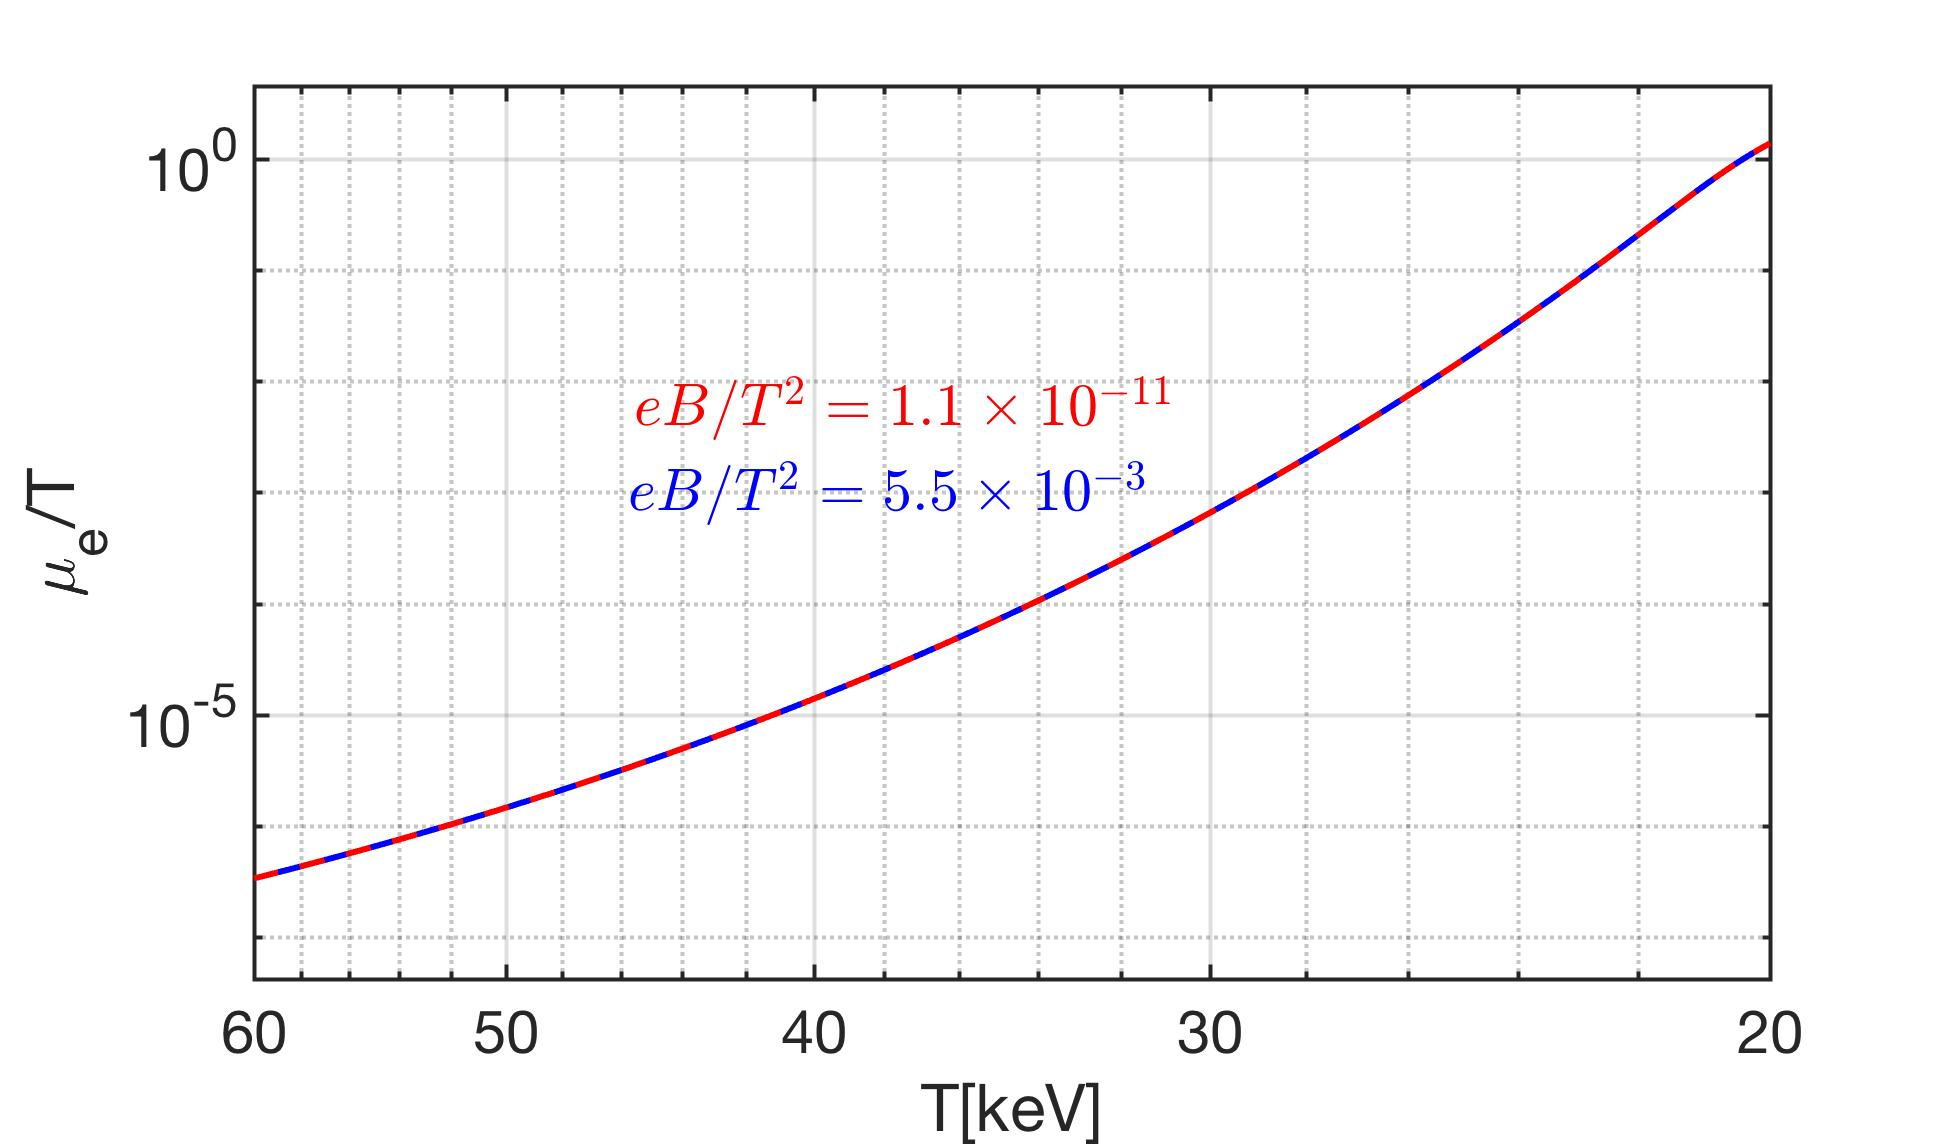
\includegraphics[width=0.5\linewidth]{ChemicalPotential_case1.jpg}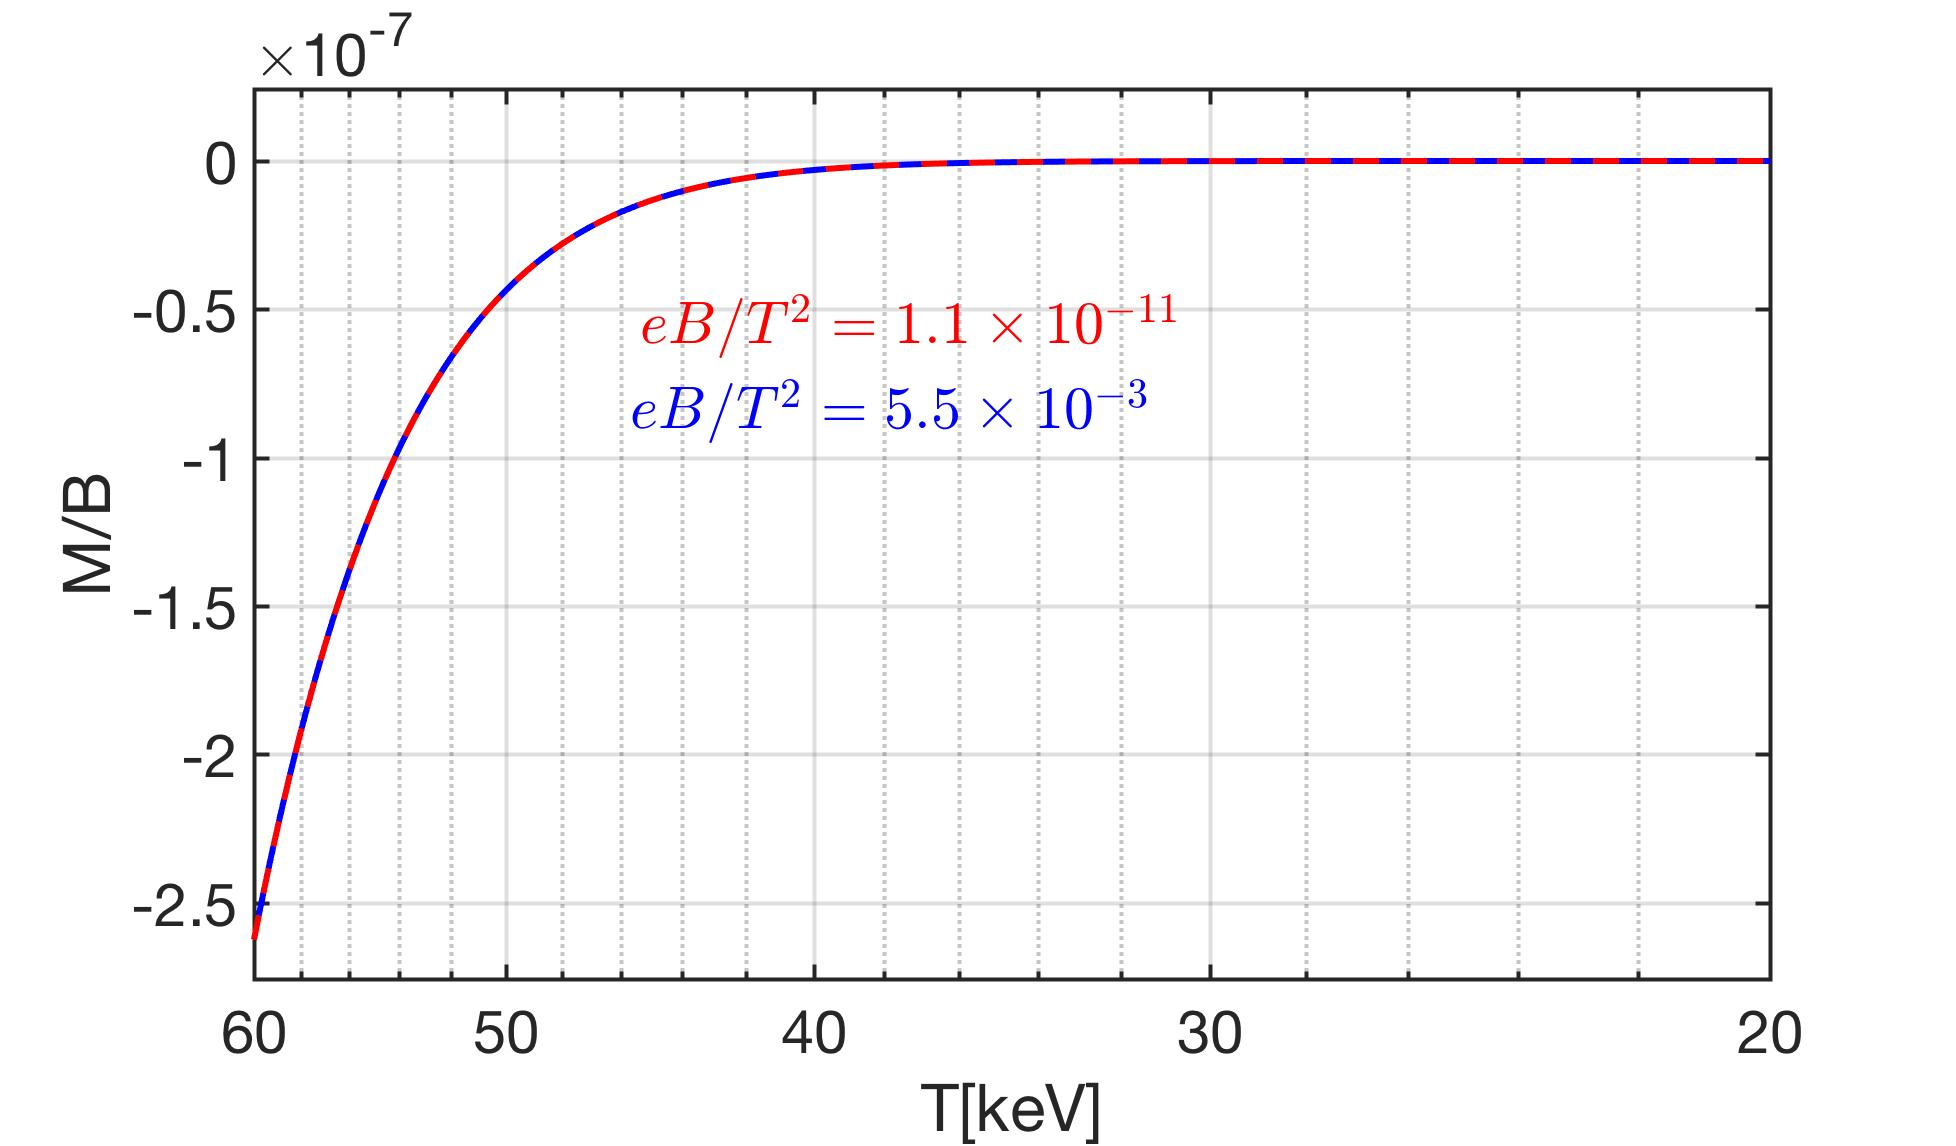
\includegraphics[width=0.5\linewidth]{Magnetization_case1.jpg}
\caption{The chemical potential $\mu_e/T$(left) and magnetization $M/B$(right) as a function of temperature $20<T<60$keV  for the case 1. The chemical potential and magnetization are not sensitive to the magnetic field, because the small value of $b_0=10^{-3}\sim10^{-8}$ can be neglected in Eq.(\ref{chemical_001}) and Eq.(\ref{Magnetization_001}). }
\label{Case1_fig} 
\end{figure}
%~~~~~~~~~~~~~~~~~~~~~~~~~~~~~~~~~~~~~~~~~~~~~~~~~~~~~~~~~~~~~~~~~~~~~~~~~~~~~~~~
  \item Case 2: $\tilde m_-=m_e$ and $x=\tilde m_-/T$,then the equations for chemical potential and magnetization can be written as
  \begin{align}\label{chemical_002}
\sinh{(\mu_e/T)}=\frac{(2\pi)^2n_p}{2T^3}\,\frac{1}{\left[x^2K_2(x)+b_0xK_1(x)+\frac{b^2_0}{6}K_0(x)\right]}
  \end{align}
and
\begin{align}\label{Magnetization_002}
\left(\frac{M}{B}\right)&=\frac{8\pi\alpha}{(2\pi)^2}\left(\frac{1}{b_0}xK_1(x)+\frac{1}{3}K_0(x)\right)\sqrt{1+\left[\frac{{(2\pi)^2n_p}/{(2T^3)}}{\left[x^2K_2(x)+b_0x K_1(x)+\frac{b^2_0}{6}K_0(x)\right]}\right]^2}
\end{align}
Using the magnetic field $b_0$ and proton density $n_p/T^3$ from pervious section, we can solve the magnetization and chemical potential  for case 2 numerically. 

In Fig {\ref{Case2_fig}}, we plot the chemical potential $\mu_e/T$(left) and magnetization $M/B$(right) as a function of temperature $T$. It shows that the chemical potential is not sensitive to the magnetic field because the small value of $b_0=10^{-3}\sim10^{-8}$ and can be neglected in Eq.(\ref{chemical_002}). However, the magnetization does depend on the magnetic field $b_0$ strongly. This is because for small magnetic field $b_0$ the dominant term in Eq(\ref{Magnetization_002}) is $xK_1(x)/b_0$. For given $b_0$, the value of magnetization can be larger than the magnetic filed, i.e. $M/B>1$  which shows the possibility that magnetic domains can be formed in early universe.

 %~~~~~~~~~~~~~~~~~~~~~~~~~~~~~~~~~~~~~~~~~~~~~~~~~~~~~~~~~~~~~~~~~~~~~~~~~~~~~~~~
\begin{figure}[h]
%\begin{center}
\centering
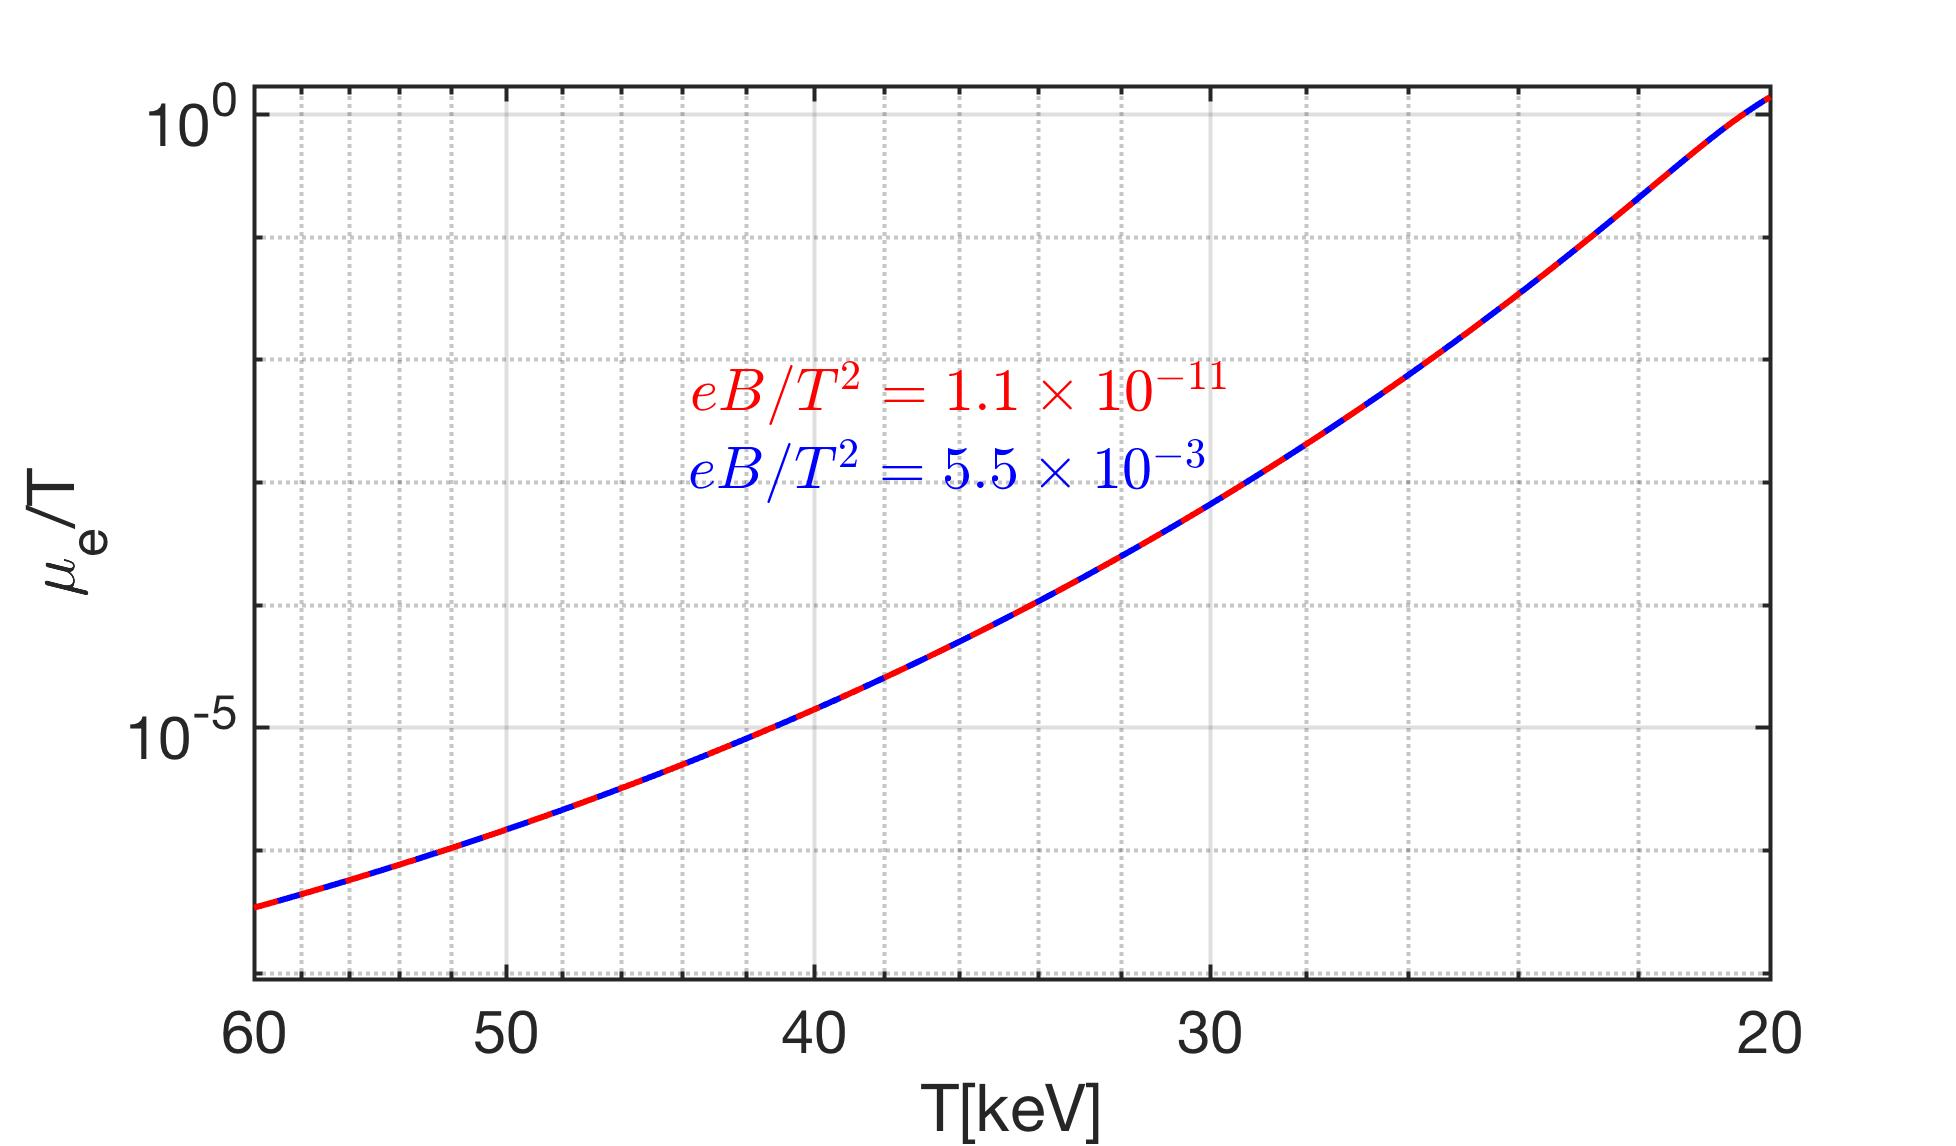
\includegraphics[width=0.5\linewidth]{ChemicalPotential_case2.jpg}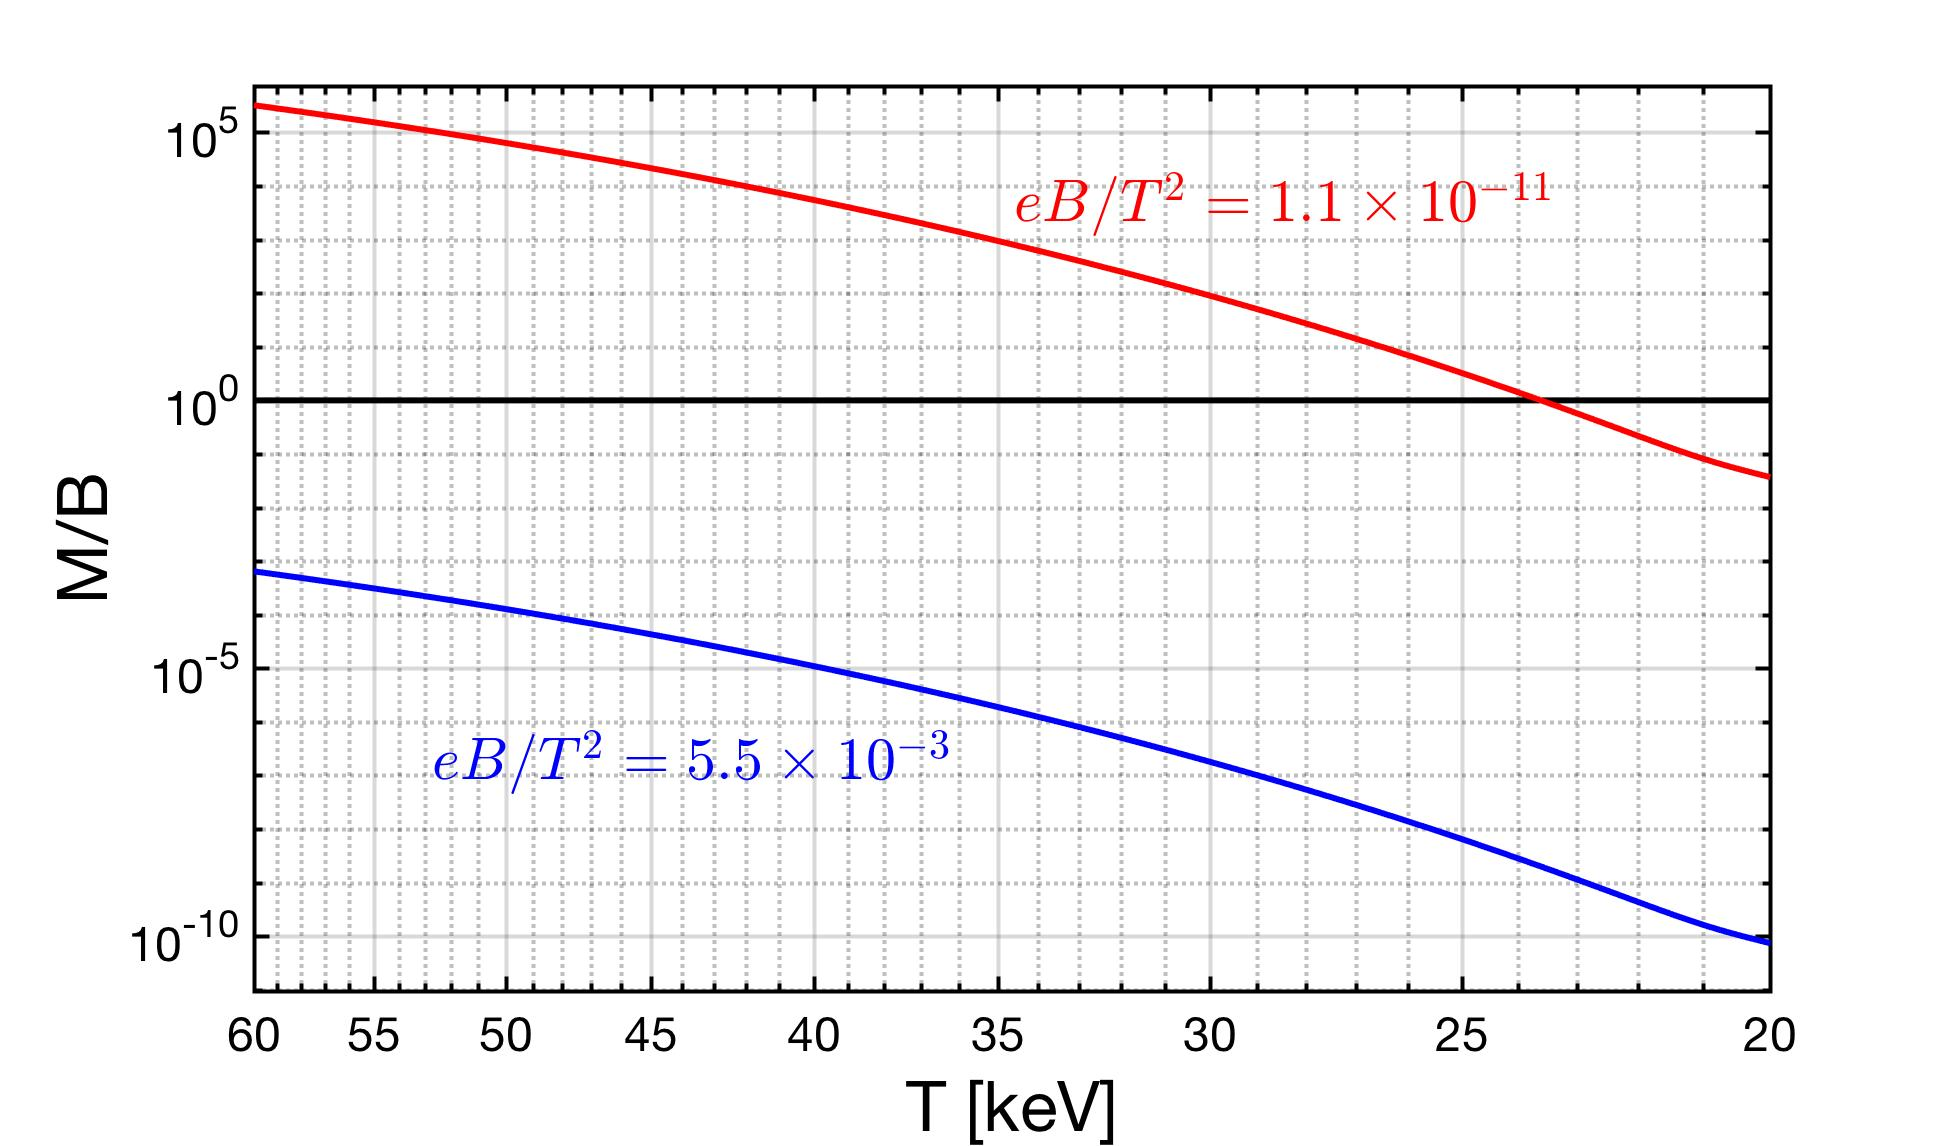
\includegraphics[width=0.5\linewidth]{Magnetization_case2.jpg}
\caption{The chemical potential $\mu_e/T$(left) and magnetization $M/B$(right) as a function of temperature $20<T<60$keV  for the case 2.  It shows that the chemical potential is not sensitive to the magnetic field $b_0$. However, the magnetization does depend on the magnetic field $b_0$ strongly. This is because for small magnetic field $b_0$ the dominant term in Eq(\ref{Magnetization_002}) is $xK_1(x)/b_0$. For giving $b_0$  we can have $M/B>1$ in early universe.}
\label{Case2_fig} 
\end{figure}
%~~~~~~~~~~~~~~~~~~~~~~~~~~~~~~~~~~~~~~~~~~~~~~~~~~~~~~~~~~~~~~~~~~~~~~~~~~~~~~~~

\end{itemize}

%~~~~~~~~~~~~~~~~~~~~~~~~~~~~~~~~~~~~~~~~~~~~~~~~~~~~~~~~~~~~~~~~~~~~~~~~~~~~~~~~~~~~~~~~~~~~~~~~~~~~~~~~~%%%%%%%%%%%%%%%%%%%%%%%%%%%%%%%%%%%%%%%%%%%%%%%%%%%%%%%%%%%%%%%%%
%%%%%%%%%%%%%%%%%%%%%%%%%%%%%%%%%%%%%%%%%%%%%%%%%%%%%%%%%%%%%%%%%
 %%%%%%%%%%%%%%%%%%%%%%%%%%%%%%%%%%%%%%%%%%%%%%%%%%%%%%%%%%%%%%%%%

\reftitle{References}
\begin{thebibliography}{99}

\bibitem{ParticleDataGroup:2022pth}
R.~L.~Workman \textit{et al.} [Particle Data Group],
``Review of Particle Physics,''
PTEP \textbf{2022}, 083C01 (2022)
doi:10.1093/ptep/ptac097

\bibitem{Kolb:1990vq} 
E.~W.~Kolb and M.~S.~Turner,
\emph{The Early Universe},
547 pp, Front.\ Phys.\ {\bf 69}, 1 (1990),
ISBN: 0201626748, 9780201626742


%\bibitem{Fromerth:2012fe}
%M.~J.~Fromerth, I.~Kuznetsova, L.~Labun, J.~Letessier and J.~Rafelski,
%``From Quark-Gluon Universe to Neutrino Decoupling: 200 < T < 2MeV,''
%Acta Phys. Polon. B \textbf{43}, no.12, 2261-2284 (2012)
%doi:10.5506/APhysPolB.43.2261
%[arXiv:1211.4297 [nucl-th]].
 

%\bibitem{Aksenov:2007}
%A. G. Aksenov, R. Ruffini, and G. V. Vereshchagin
%``Thermalization of Nonequilibrium Electron-Positron-Photon Plasmas,''
%Phys.\ Rev.\ Lett.\ \textbf{99}, 125003 (2007) 
%doi: 10.1103/PhysRevLett.99.125003

%\bibitem{Aksenov:2010}
%A. G. Aksenov, R. Ruffini, and G. V. Vereshchagin
%``Pair plasma relaxation time scales''
%Phys.\ Rev.\ E \textbf{81}, 046401 (2010)
%doi: 10.1103/PhysRevE.81.046401
\end{thebibliography}

%%%%%%%%%%%%%%%%%%%%%%%%%%%%%%%%%%%%%%%%%%
\end{document}
